%%%%%%%%%%%%%%%%%%%%%%%%%%%%%%%%%%%%%%%%%%%%%%%%%%%%%%%%%%%%%%%%%%%
%                                                                 %
%                            CHAPTER TWO                          %
%                                                                 %
%%%%%%%%%%%%%%%%%%%%%%%%%%%%%%%%%%%%%%%%%%%%%%%%%%%%%%%%%%%%%%%%%%%
\chapter{RELATED WORKS} \label{sec:related}

% Make a TLDR 
The online architectural sketching interface for simulations (OASIS) is an alternative interface for key algorithms originally developed for the Virtual Heliodon.  The Virtual Heliodon is a spatial augmented tangible user interface for daylighting analysis.  Both the Virtual Heliodon and OASIS rely on the physical sketch interpretation algorithm and the daylight rendering engine.  The physical sketch interpretation algorithm is used to convert physical sketches, in the Virtual Heliodon's tangible user interface, to water-tight triangle meshes.  These triangle meshes are then used as input for the daylight rendering engine.  The daylight rendering engine is a scalable renderer that uses GPU-accelerated photon mapping to produce daylight visualizations at interactive frame rates.  Furthermore, while there are many well established architectural tools for daylight analysis, there exist only a handful of tools that are used in the early stages of design.  We will discuss how both OASIS and the Virtual Heliodon share common goals with some of these more popular daylight analysis tools. \\

\section{Virtual Heliodon}


The Virtual Heliodon is a spatial augmented reality system with a tangible user interface for the early collaborative design of interior spaces with daylighting \cite{sheng2009virtual, cutler2009inferring,nasman2013physical}.  The Virtual Heliodon is composed of multiple projectors, a circular table, and a collection of foam primitives.  A large frame holds the projectors above the table top at evenly spaced intervals.  These projectors all face towards the table top at the center of the system; The configuration of the Virtual Heliodon is shown below in Figure-\ref{fig:virtual_heliodon} This tangible user interface lets users physically engage with wall primitives.  Users can define architectural spaces by moving and rotating wall primitives on the table top.  Some architectural spaces created on the Virtual Heliodon are shown in Figure-\ref{fig:heliodon_sketch}.  After the creation of a physical sketch, a network of computers use projectors to superimpose daylight renderings onto foam primitives placed on the table top.  The Virtual Heliodon requires multiple projectors in varying positions along the frame to superimpose renderings onto all of the wall primitives.  Projecting daylight renderings directly onto wall primitives creates an augmented reality environment that gives users a sense of immersion \cite{nasman2013physical}.  The Virtual Heliodon has gone through a few evaluations and has
been shown to be engaging and valuable as an educational daylighting tool \cite{nasman2013physical}. \\

% Figures
\begin{figure}[h]
\centering
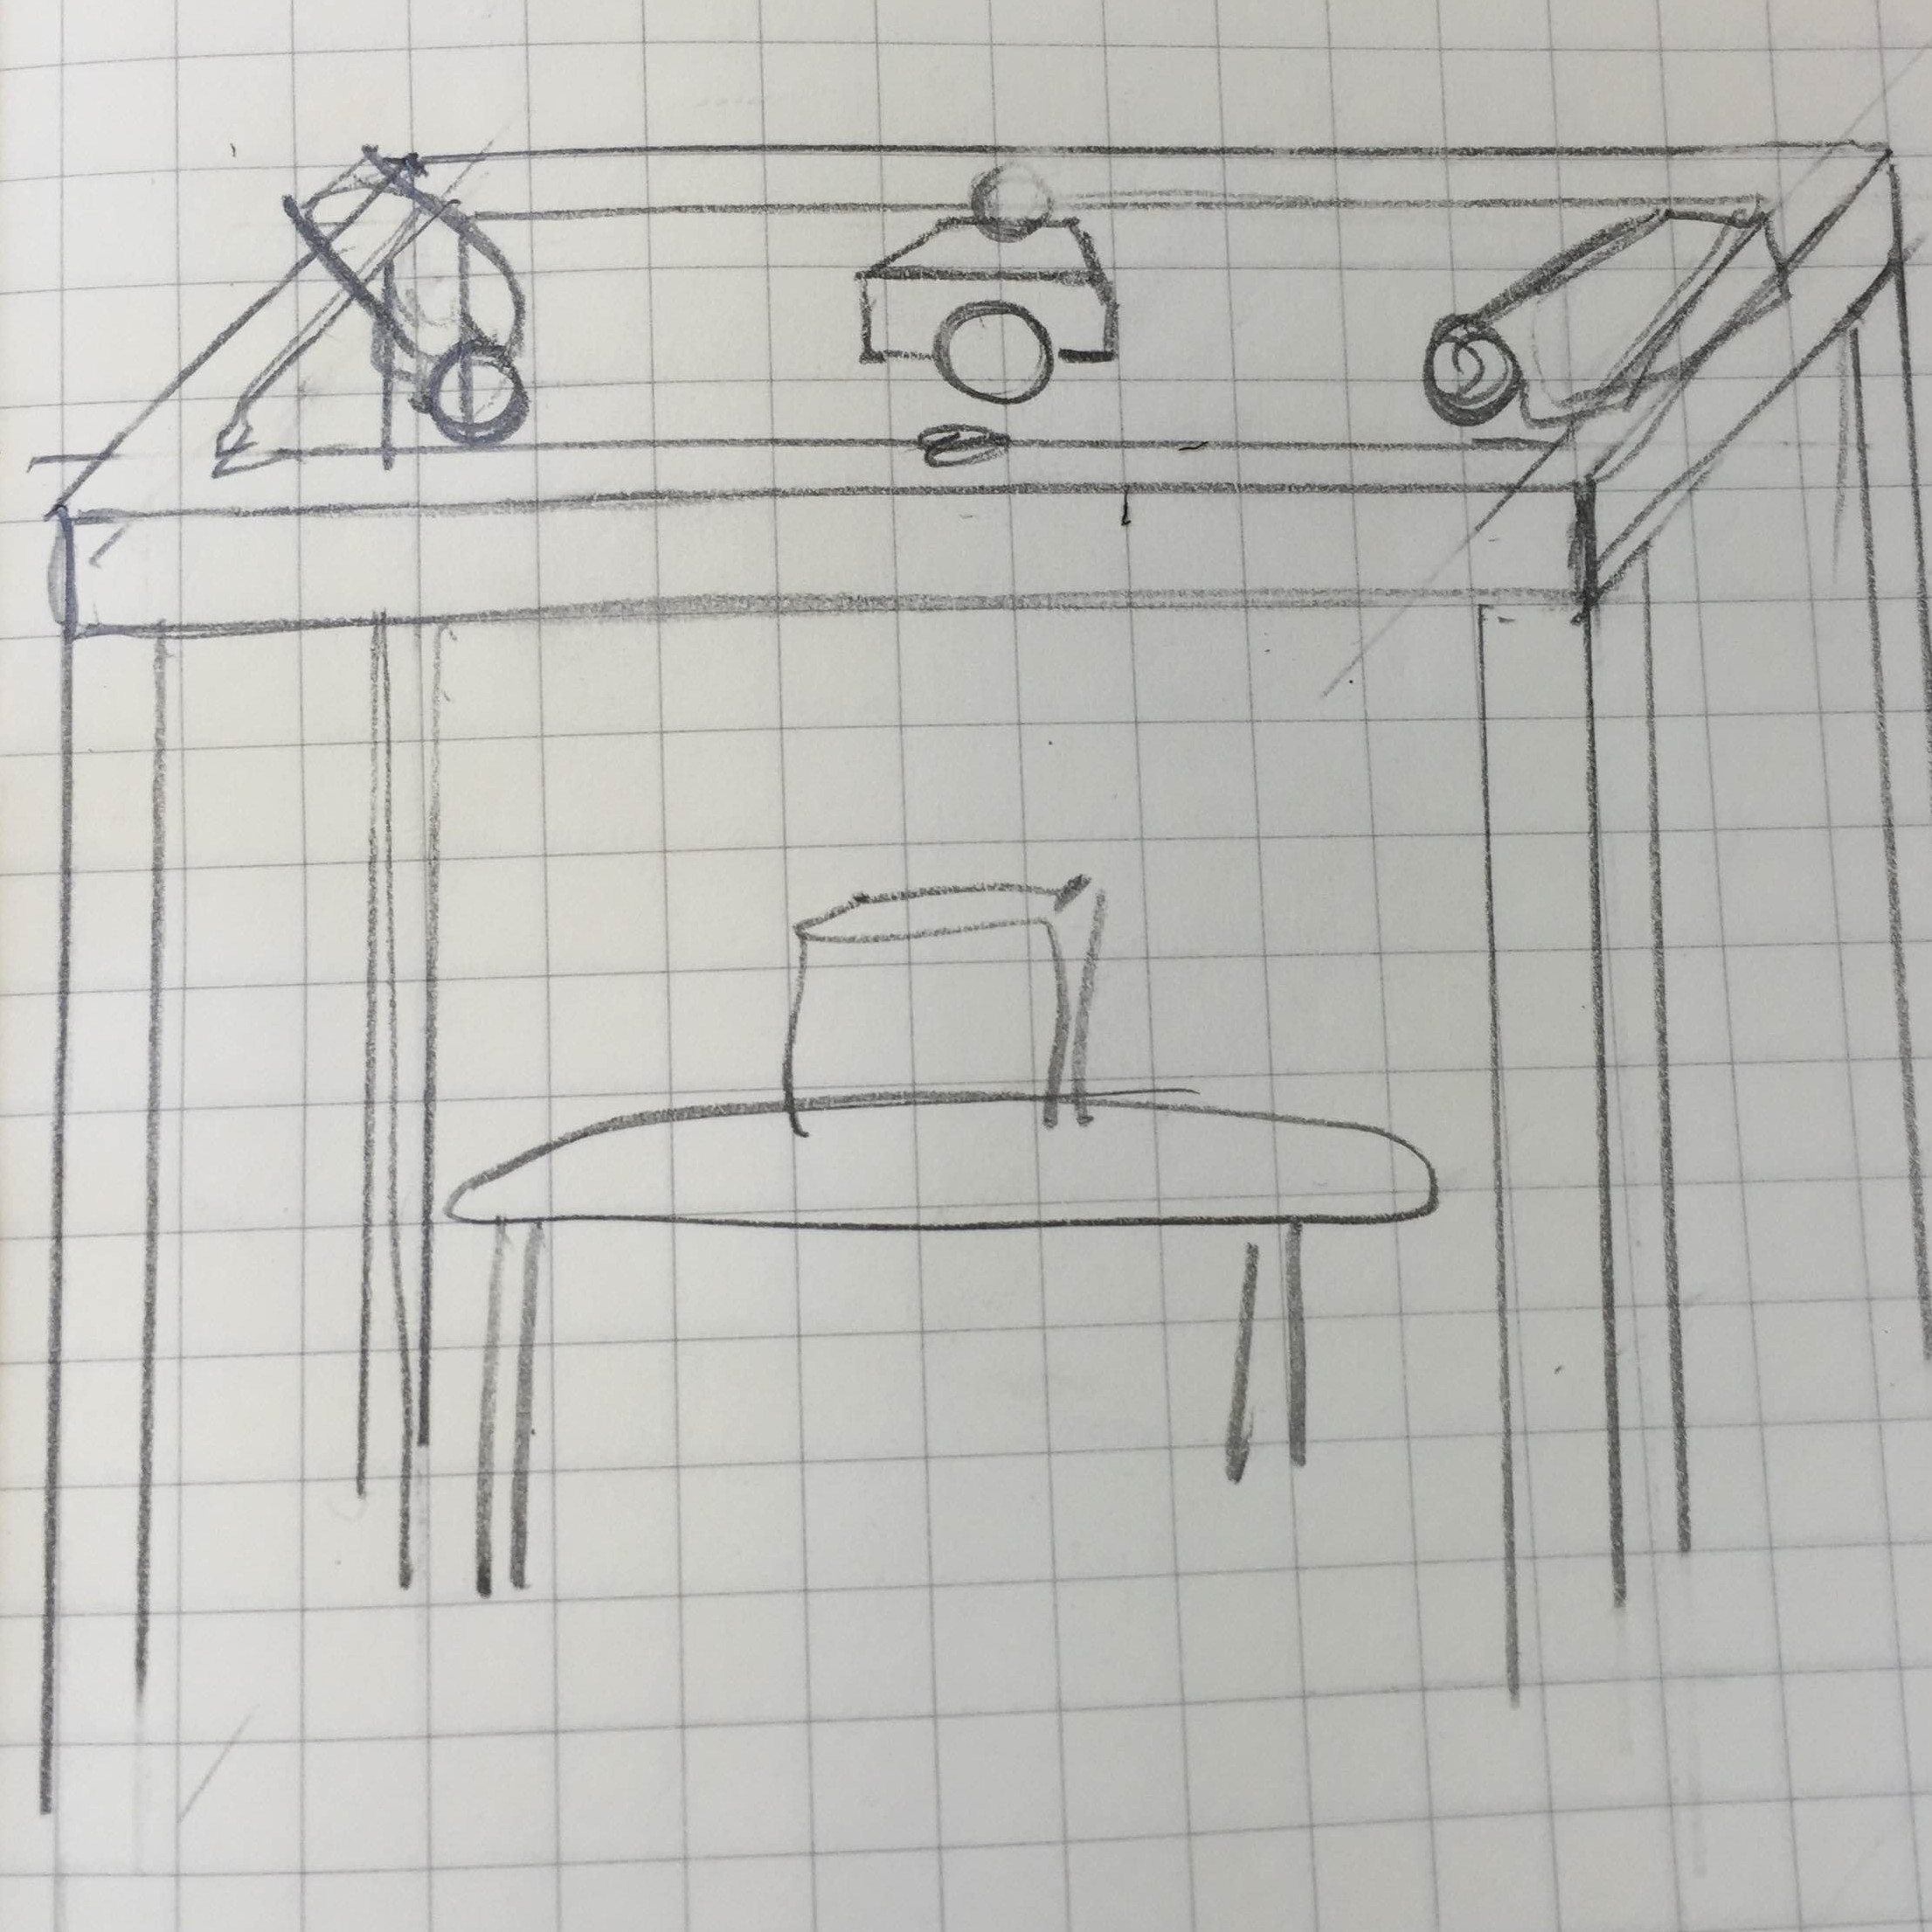
\includegraphics[width=0.5\textwidth]{virtual_heliodon}
\caption[Overiew of the Virtual Heliodon.]{Overview of the Virtual Heliodon. Note the projector arrangement and table at the center.}
\label{fig:virtual_heliodon}
\end{figure}

\begin{figure}[h]
\centering
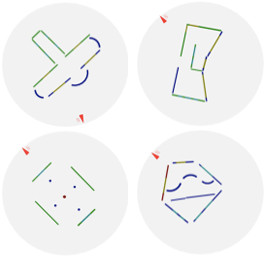
\includegraphics[width=0.5\textwidth]{heliodon_sketch}
\caption{Example physical sketches created by users on the Virtual Heliodon.}
\label{fig:heliodon_sketch}
\end{figure}

\section{Physical Sketch Interpretation Algorithm}

A previous study evaluated the effectiveness of the physical sketch interpretation algorithm used in the Virtual Heliodon \cite{cutler2009inferring}.  This study compared users' intended interpretation of physical sketches to both the interpretation from the physical sketch interpretation algorithm and human subjects.  In brief, the study concluded that on average the physical sketch interpretation algorithm matched users' intention 78\% of the time given non-ambiguous models \cite{cutler2009inferring}.  Aside from ambiguous sketches, the Virtual Heliodon provided reliable 3D geometries that matched users' intended floor plan designs.  For this reason OASIS uses the same physical sketching interpretation algorithm employed in the Virtual Heliodon.\\

Interpreting sketches is not the only method of turning concepts into 3D models.  Traditionally, both parametric and geometric modeling are used to create 3D models of architectural spaces.  Daylight analysis tools such as the Home Energy Efficient Design tool (HEED)\footnote{http://www.energy-design-tools.aud.ucla.edu/[Access: Apr 8 2016]} and eQuest\footnote{http://www.doe2.com/equest/[Access: Apr 8 2016]} use parametric modeling to generate 3D models of architectural spaces.  Parametric modeling is the creation of a model from a template by specifying parameters such as wall lengths, walls heights, and window positions through numerical entry.  Both HEED and eQuest are intended for use in the schematic design phase and offer a large variety of energy analysis measurements.  Due to the high cost of effort in parametrically designing an architectural space, both HEED and eQUEST feature wizards to guide users through the process.  Specifically, HEED allows users to ``draw'' the floor plan of a building by filling in a 2D square grid. Filled in portions of the grid are used to define the floor plan of a building. The main disadvantage of this interface is the limitation of only supporting axis aligned models.  Additionally, the interface on eQUEST only allows users to pick from a small set of template models including rectangular models, L shaped models, and U shaped models.\\ 

On a related note, geometric modeling is another 3D modeling approach commonly used to create complex architectural designs in software.  Geometric modeling gives users the ability to create 3D objects by modifying basic shapes visually.  The process of geometrically modeling a conceived architectural space in software is non-trivial.  Being able to geometrically model complex 3D geometries is an art that requires precision and a deep understanding of the geometric tools available.  As a result, the modeling of architectural designs in software is usually pushed back into the design development phase, where there are fewer large changes in design \cite{Galasiu}.  SketchUp and AutoDesk\footnote{http://www.autodesk.com/[Accessed: Apr 8 2016]} are both popular architectural design tools that use geometric modeling for the generation of architectural spaces. \\

In practice, sketching is still used during the early design phase of architecture because of the unmatched speed \& efficiently it offers designers \cite{Galasiu}.  Architectural sketching interfaces were developed as an alternative to parametric and geometric modeling.  LightSketch and the VR SketchPad project both use an architectural sketching interface \cite{do2001vr,glaser2003sketch}.  Specifically, LightSketch shares much in common with OASIS.  LightSketch gives users the ability to draw walls, windows, and interior lighting elements in order to create 3D architectural spaces \cite{glaser2003sketch}; the 2D drawings are then interpreted and turned into 3D models through different methods than the Virtual Heliodon's physical sketch interpretation algorithm.  Users can then perform daylight analysis and generate renderings from those 3D models on LightSketch.  LightSketch uses Radiance as it's daylight rendering engine and as a result renderings can take several minutes to complete.  LightSketch, however, is limited to shoe-box\footnote{Shoe-box is a term used to generalize rooms that are rectangular prisms in shape.} geometries.  Users cannot freely design non shoe-box floor plans, as is possible in the VR SketchPad project and the Virtual Heliodon.  The VR SketchPad project supports the creation of a wide variety of 3D models for early visualization and exploration of architectural spaces \cite{do2001vr}.  Also, VR SketchPad project was available as an online tool, similar to OASIS.  The tool also supported a broad vocabulary of furniture item.  Users could draw furniture items into the scene using this vocabulary and the VR SketchPad project would interpret the furniture drawings and choose the appropriate 3D furniture models to place into the scene.  A limitation of the 3D models generated from the VR SketchPad project is that the models are only extrapolated from drawn sketches and as a result cannot be used for simulations.  Explicitly, the VR SketchPad project does not distinguish between interior and exterior spaces in a design but instead generates objects only where users sketch them.  On the other hand, sketches in the Virtual Heliodon and OASIS get converted into water-tight models that are required for daylight simulations.\\

\section{Daylight Rendering Engine}

% <Explanation of how DRE works>
In addition to using the Virtual Heliodon's physical sketch interpretation algorithm, I also use the Virtual Heliodon's daylight rendering engine \cite{li2011photon,nasman2013physical}.  The daylight rendering engine takes advantage of NVidia's Optix GPU ray tracing framework for the parallelization of photon mapping \cite{parker2010optix}.  The daylight rendering engine is specialized to provide viewpoint independent daylight renderings at interactive rates.  Photon mapping is the approximation of global illumination by tracing rays outward from emitters and then gathering photons after several bounces to calculate indirect illumination per triangle or patch \cite{hachisuka2008progressive}.  Window panes are considered emitters our daylight rendering engine; windows in our system emit both direct sunlight and diffuse skylight.  When photons are emitted from the window pane their position and direction are chosen at random; However, the intensity of an emitted photon is determined by its direction as defined by the appropriate International Commission on Illumination's (CIE) sky model \cite{matsuura1988luminance}.  An addition a non-recursive ray tracing procedure is used to take into consideration the hard edges of illumination caused from direct sun light. \\
	% </Explanation of how DRE works>

	% <Why we choose to use the Daylight Rendering Engine>
	% It is fast
	% It was in house (worked with our current pipeline)
	% It is scalable to multiple machines via MPI
I choose to use the Virtual Heliodon's daylight rendering engine over other alternatives because of three reasons.  Firstly, the daylight rendering engine provided daylight renderings at interactive rates. Many alternatives available at the time required minutes to create clear daylight renderings. As an early design tool, providing renderings to designers as quickly as possible is crucial for the iterative creative design process.  Secondly, the Virtual Heliodon's daylight rendering engine was optimized to work along side the Virtual Heliodon's physical sketch interpretation algorithm. The existence of a pipeline between both of these components was valuable as it provided an existing base for our online sketching interface. Additionally, I had unrestricted access to the Virtual Heliodon's code base which would allow me to extend the daylight rendering engine if needed. Unrestricted access to the source of code alternative daylighting tools is not always possible.  Lastly, the daylight rendering engine has an optional message passing (MPI) interface that would allow us to scale OASIS. As of right now, OASIS does not use this MPI, but should we choose to generate more detailed rendering at similar interactive rates the option of using multiple graphics cards to accelerate rendering is available. \\
	% </Why we choose to use the Daylight Rendering Engine>

	% < Our tool compared to industry standard >
Although I did choose to use the Virtual Heliodon's daylight rendering engine, I was aware of Radiance; Radiance is the long-standing industry standard for daylight rendering.  Moreover, radiance is a command line tool that comes packaged with many daylighting metrics and visualization options.  However, the lack of an graphical user interface makes Radiance hard to use for non-experts; as a result many daylight analysis tools a provide graphical interface for Radiance.  More importantly Radiance is an industry standard because it is one of the few daylight rendering engines that has been validated \cite{mcneil2013validation}. While, the Virtual Heliodon's daylight rendering engine has not been directly validated against Radiance, the rendering engine has been validated against a radiosity based rendering engine.  This radiosity based rendering engine, used in previous versions of the Virtual Heliodon, was validated against Radiance \cite{sheng2010global}.  I choose to use the Virtual Heliodon's daylight rendering engine because at the time Radiance required more time to produce clear and noise-free results than the Virtual Heliodon \cite{compagnon1997radiance}.  Currently research on GPU accelerated implementation of Radiance are being developed that significantly increase performance of Radiance \cite{zuo2012acceleration}.  In the future I will look into these GPU implementations of radiance to examine if their integration into OASIS is viable and effective.  \\

% </ Our tool compared to industry standard > 

All things considered, the Virtual Heliodon's daylight rendering engine meets our needs in OASIS as a fast scalable in-house rendering engine for qualitative and quantitative daylight analysis during the early stages of design.

\section{Related Software}

% Read for grammar
% Add in Barb's fixes
% Restructure 

% <Vasari>
OASIS shares goals in common with other daylight analysis software.  Increased value on sustainability and energy efficiency drives the development of early design tools for daylight and performance analysis.  One such piece of software is AutoDesk's latest early design tool, Project Vasari\footnote{http://autodeskvasari.com/[Accessed: Apr 8 2016]}.  Project Vasari is a stand alone geometric modeling software with an interface similar to AuthoDesk's Revit\footnote{http://www.autodesk.com/products/revit-family/[Accessed: Apr 8 2016]}.  Project Vasari, unlike Revit, was designed for energy analysis during the conceptual design of architectural spaces.  Project Vasari comes packaged with a suite of energy analysis visualizations, including several daylighting visualizations.\\
% </Vasari>

% <Plug ins>
Most major architectural design tools support energy analysis plug-ins; These plug-ins come packaged with a variety of energy metrics and visualizations, including daylighting visuals.  A tool with similar features to Project Vasari is Ecotect\footnote{http://usa.autodesk.com/ecotect-analysis/[Access: Apr 8 2016]} -- an AutoDesk plug-in.  Ecotect offers a collection of useful visualizations such as sun paths, building shadow previews, and daylighting factor visuals. \\

SketchUp is another notable conceptual design tool that does not directly support energy analysis or advance daylighting features\footnote{http://www.sketchup.com/[Accessed: Apr 8 2016]}; however there are a handful of plug-ins for SketchUp that do.  For example VE-Ware by IES is a free energy plug-in for SketchUp and Revit.  Given a model created in SketchUp VE-Ware will generate detailed energy analysis reports.  Also, another noteworthy SketchUp extension is Lightsolve \cite{andersen2008intuitive}.  While Lightsolve is not officially a SketchUp plug-in, LightSolve does support importing models directly from SketchUp.  LightSolve is noteworthy because its main focus is on daylight analysis.  Lightsolve is an early design daylight analysis tool that gives designers both annual metrics and qualitative renderings.  Specifically, within the application designers can analyze both quantitative illumination metrics and view renderings from multiple viewpoints simultaneously.  Lightsolve also provides visuals on the sun's position and elevation information on the same page as the daylighting metrics and renderings.  All of these visual elements on the same display offers designers a better understanding of the daylighting conditions within their design \cite{andersen2011informing}. \\ 

Lastly, Rhinoceros\footnote{https://www.rhino3d.com/[Accessed: Apr 8 2016]} is a general 3D Modeling tool commonly used for creating non-axis aligned architectural models and supports plug-ins such as LadyBug for basic energy analysis \cite{ladybug}.  LadyBug supports a wide variety of energy analysis visualizations, but only has a few visualizations specific to daylighting analysis -- including sun path visuals and hourly radiation studies in real time. \\ % <Plug ins>

On the whole, all of these tools offer rich and informative daylighting analysis during the conceptual  design of architectural spaces.  However they all rely on geometrically created models.  During the early design stage of architectural design, the ability to express concepts as 3D models quickly is invaluable.  As a result , researchers have investigated faster and initiative methods to generate 3D models for daylighting analysis.  \\

\section{Chapter Summary}

In OASIS I use both the Virtual Heliodon's daylight rendering engine and the physical sketch interpretation algorithm.  In order to understand why I use both of these key components, the original purpose of each component must be made clear.  The physical sketch interpretation algorithm was originally used to convert physical sketches into 3D water-tight triangle meshes for use in the daylight rendering engine.  The daylight rendering engine's initial purpose was to generate daylight renderings and produce texture images that would be superimposed onto physical sketches.  This method provided users a view point independent visualization of daylight within an architectural space.  While there were other daylight rendering engine alternatives, we choose to use the Virtual Heliodon's native rendering engine for its speed, compatibility, and scalability.  Moreover, there are a variety of related daylight analysis tools from which architects can choose from.  However, very few tools concentrate on the early design stage of architectural design.  OASIS is not the most fully featured architectural modeling tool; however, it is one of the few early design tools that features a sketching interface. \\
